
% ============================================================
% APPENDIX D -- Field Mapping Additional Results
% ============================================================

This appendix presents the complete set of magnetic field mapping figures for all fixture coordinates measured during the clinical session at \gls{bergan}. The main text discusses the results at coordinate G6 in detail, as it served as the primary reference coordinate for the translational force analysis (Section~\ref{sec:resClinicTrans}). The figures here extend the field presentation to all six sampled coordinates: 00, A3, A6, D3, G3, and G6 (Figure \ref{fig:mapPlat_grid}). For each coordinate, three quantities are shown as a function of axial position: magnetic flux density B, spatial gradient dB/dz, and the force-relevant product B times grad B. A summary figure comparing all coordinates is included at the end. These results also support the cross-coordinate force ratio predictions reported in Figure~\ref{fig:comparison_ordinate}.



\begin{figure}[h!]
	\centering
	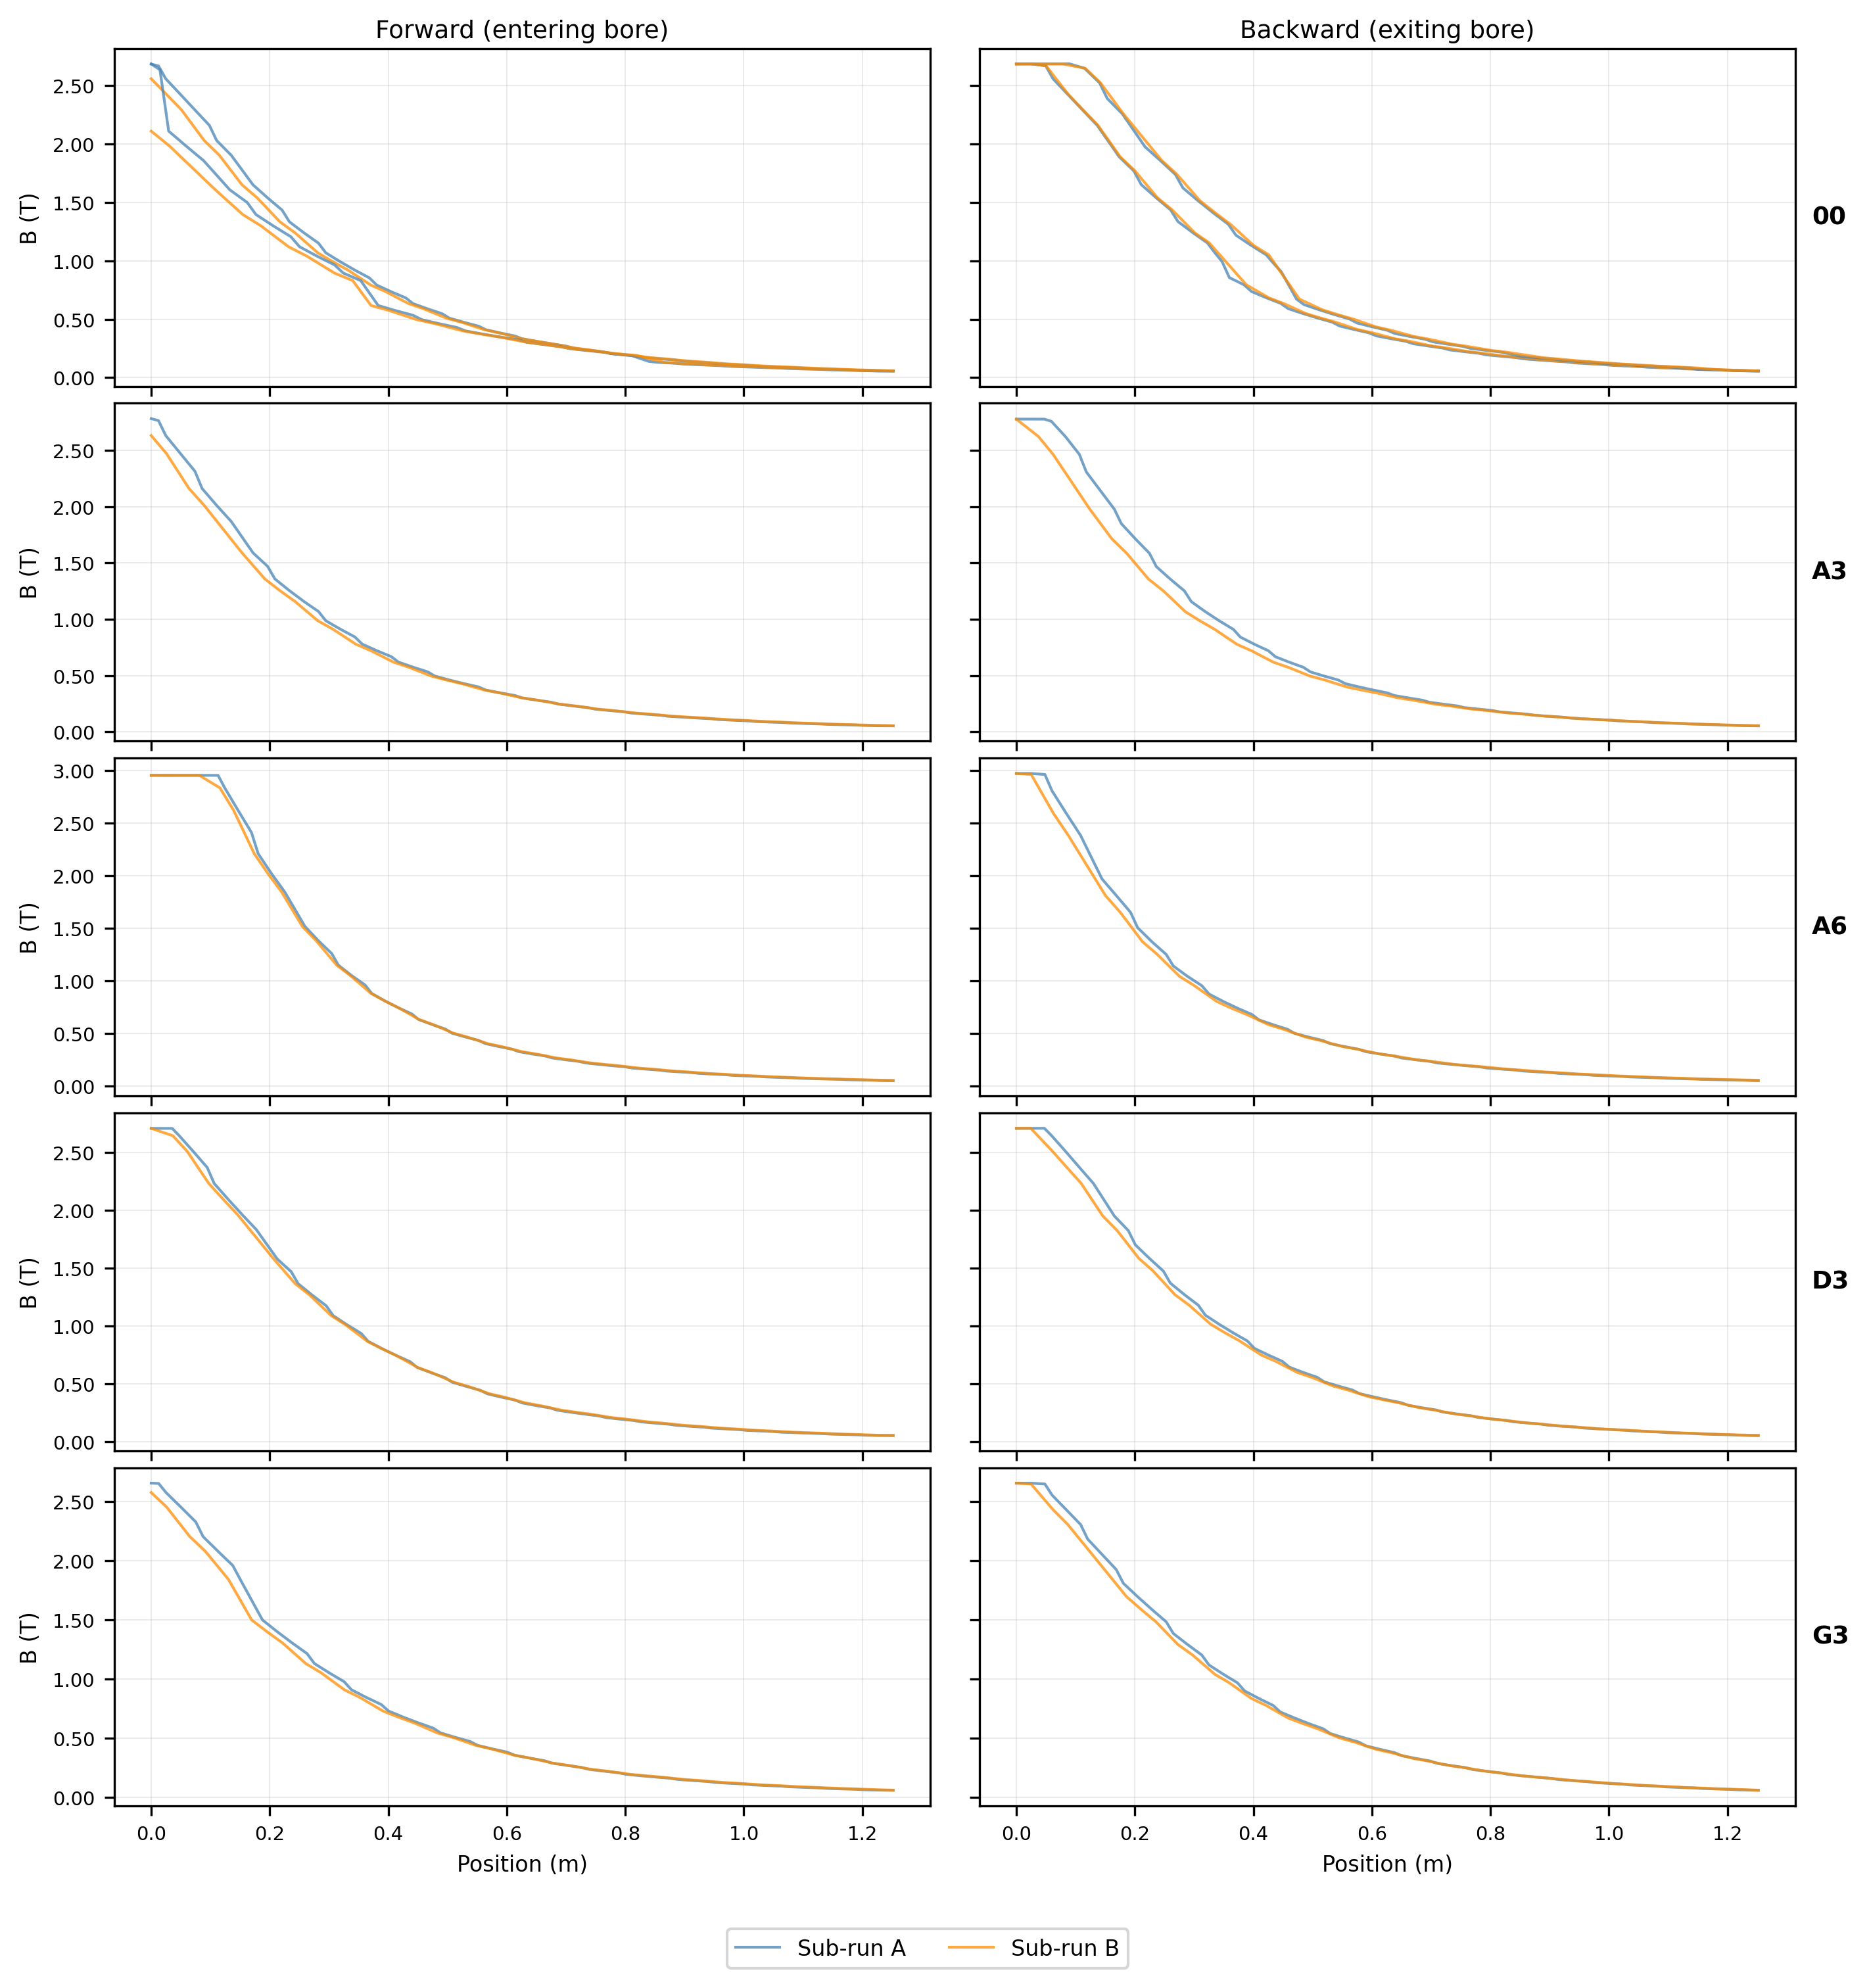
\includegraphics[width=0.95\textwidth]{Assets/allCoords_betterPlots/summary_B.png}
	\caption[Magnetic field at all positions separately]{Magnetic field along the measurement path.}
	\label{fig:allCoords_B}
\end{figure}

\begin{figure}[h!]
	\centering
	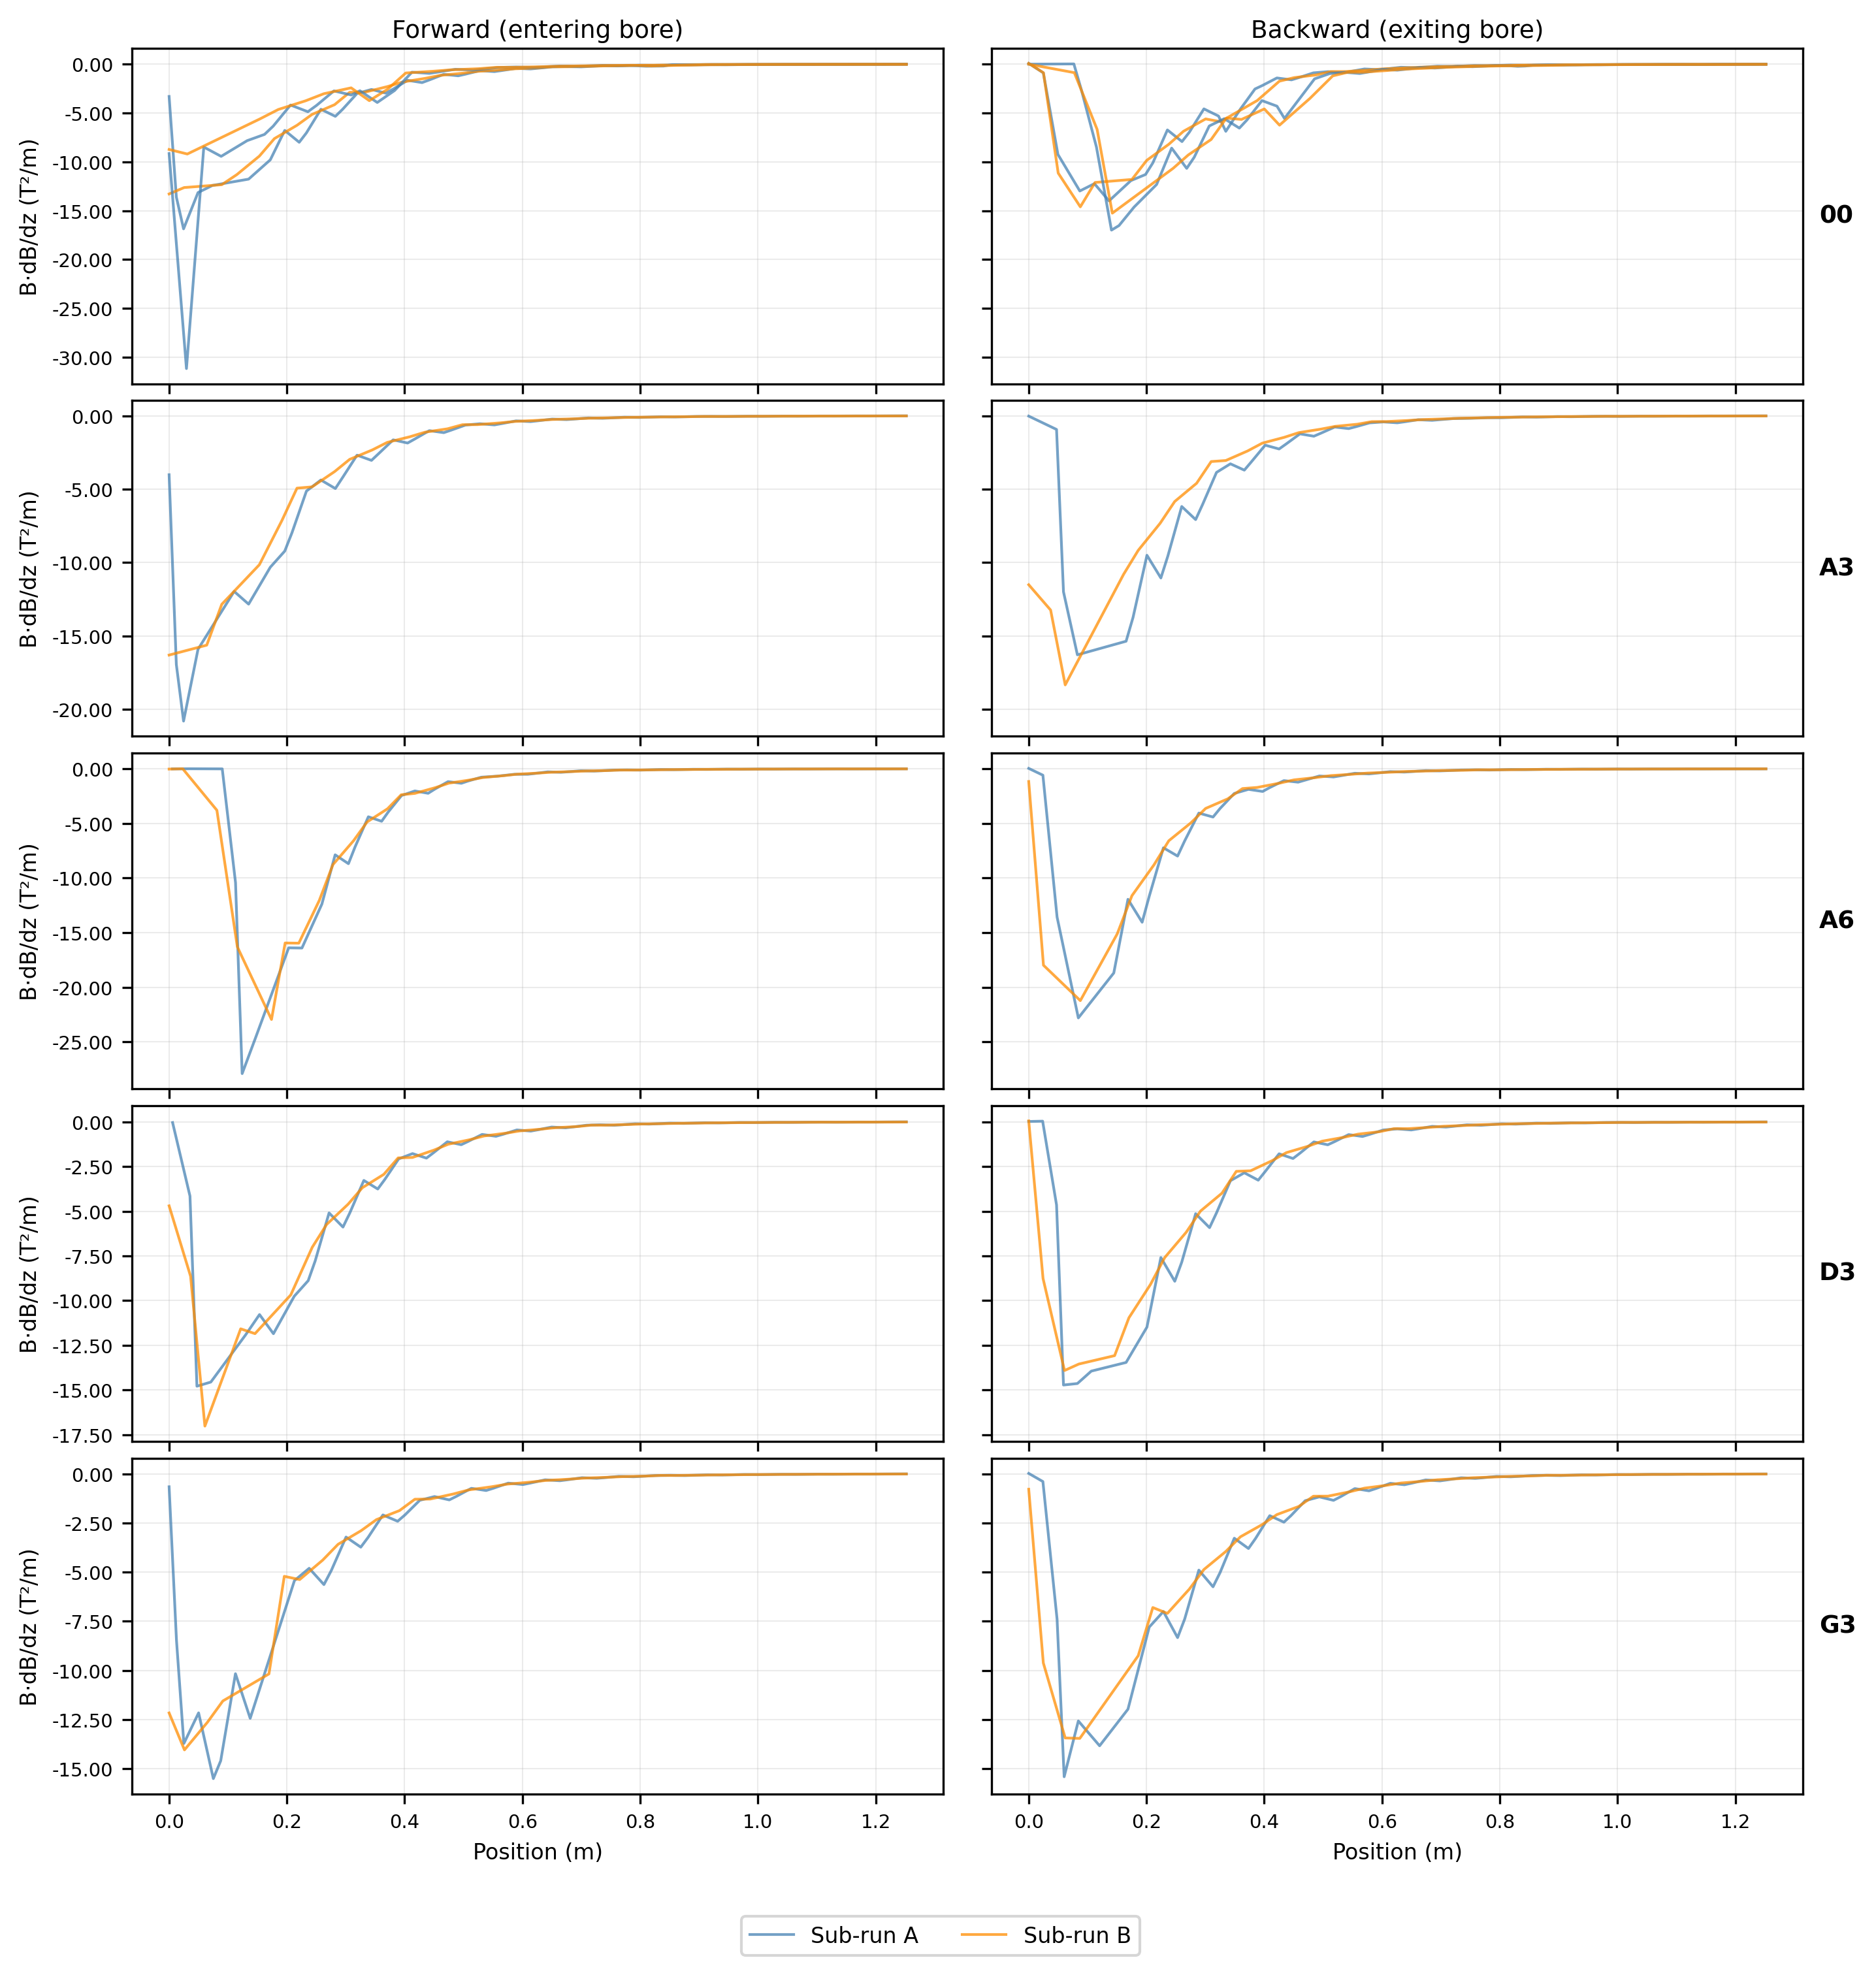
\includegraphics[width=0.95\textwidth]{Assets/allCoords_betterPlots/summary_BgradB.png}
	\caption[Magnetic field spatial gradient at all positions separately]{Magnetic field spatial gradient along the measurement path}
	\label{fig:allCoords_gradB}
\end{figure}


\begin{figure}[h!]
	\centering
		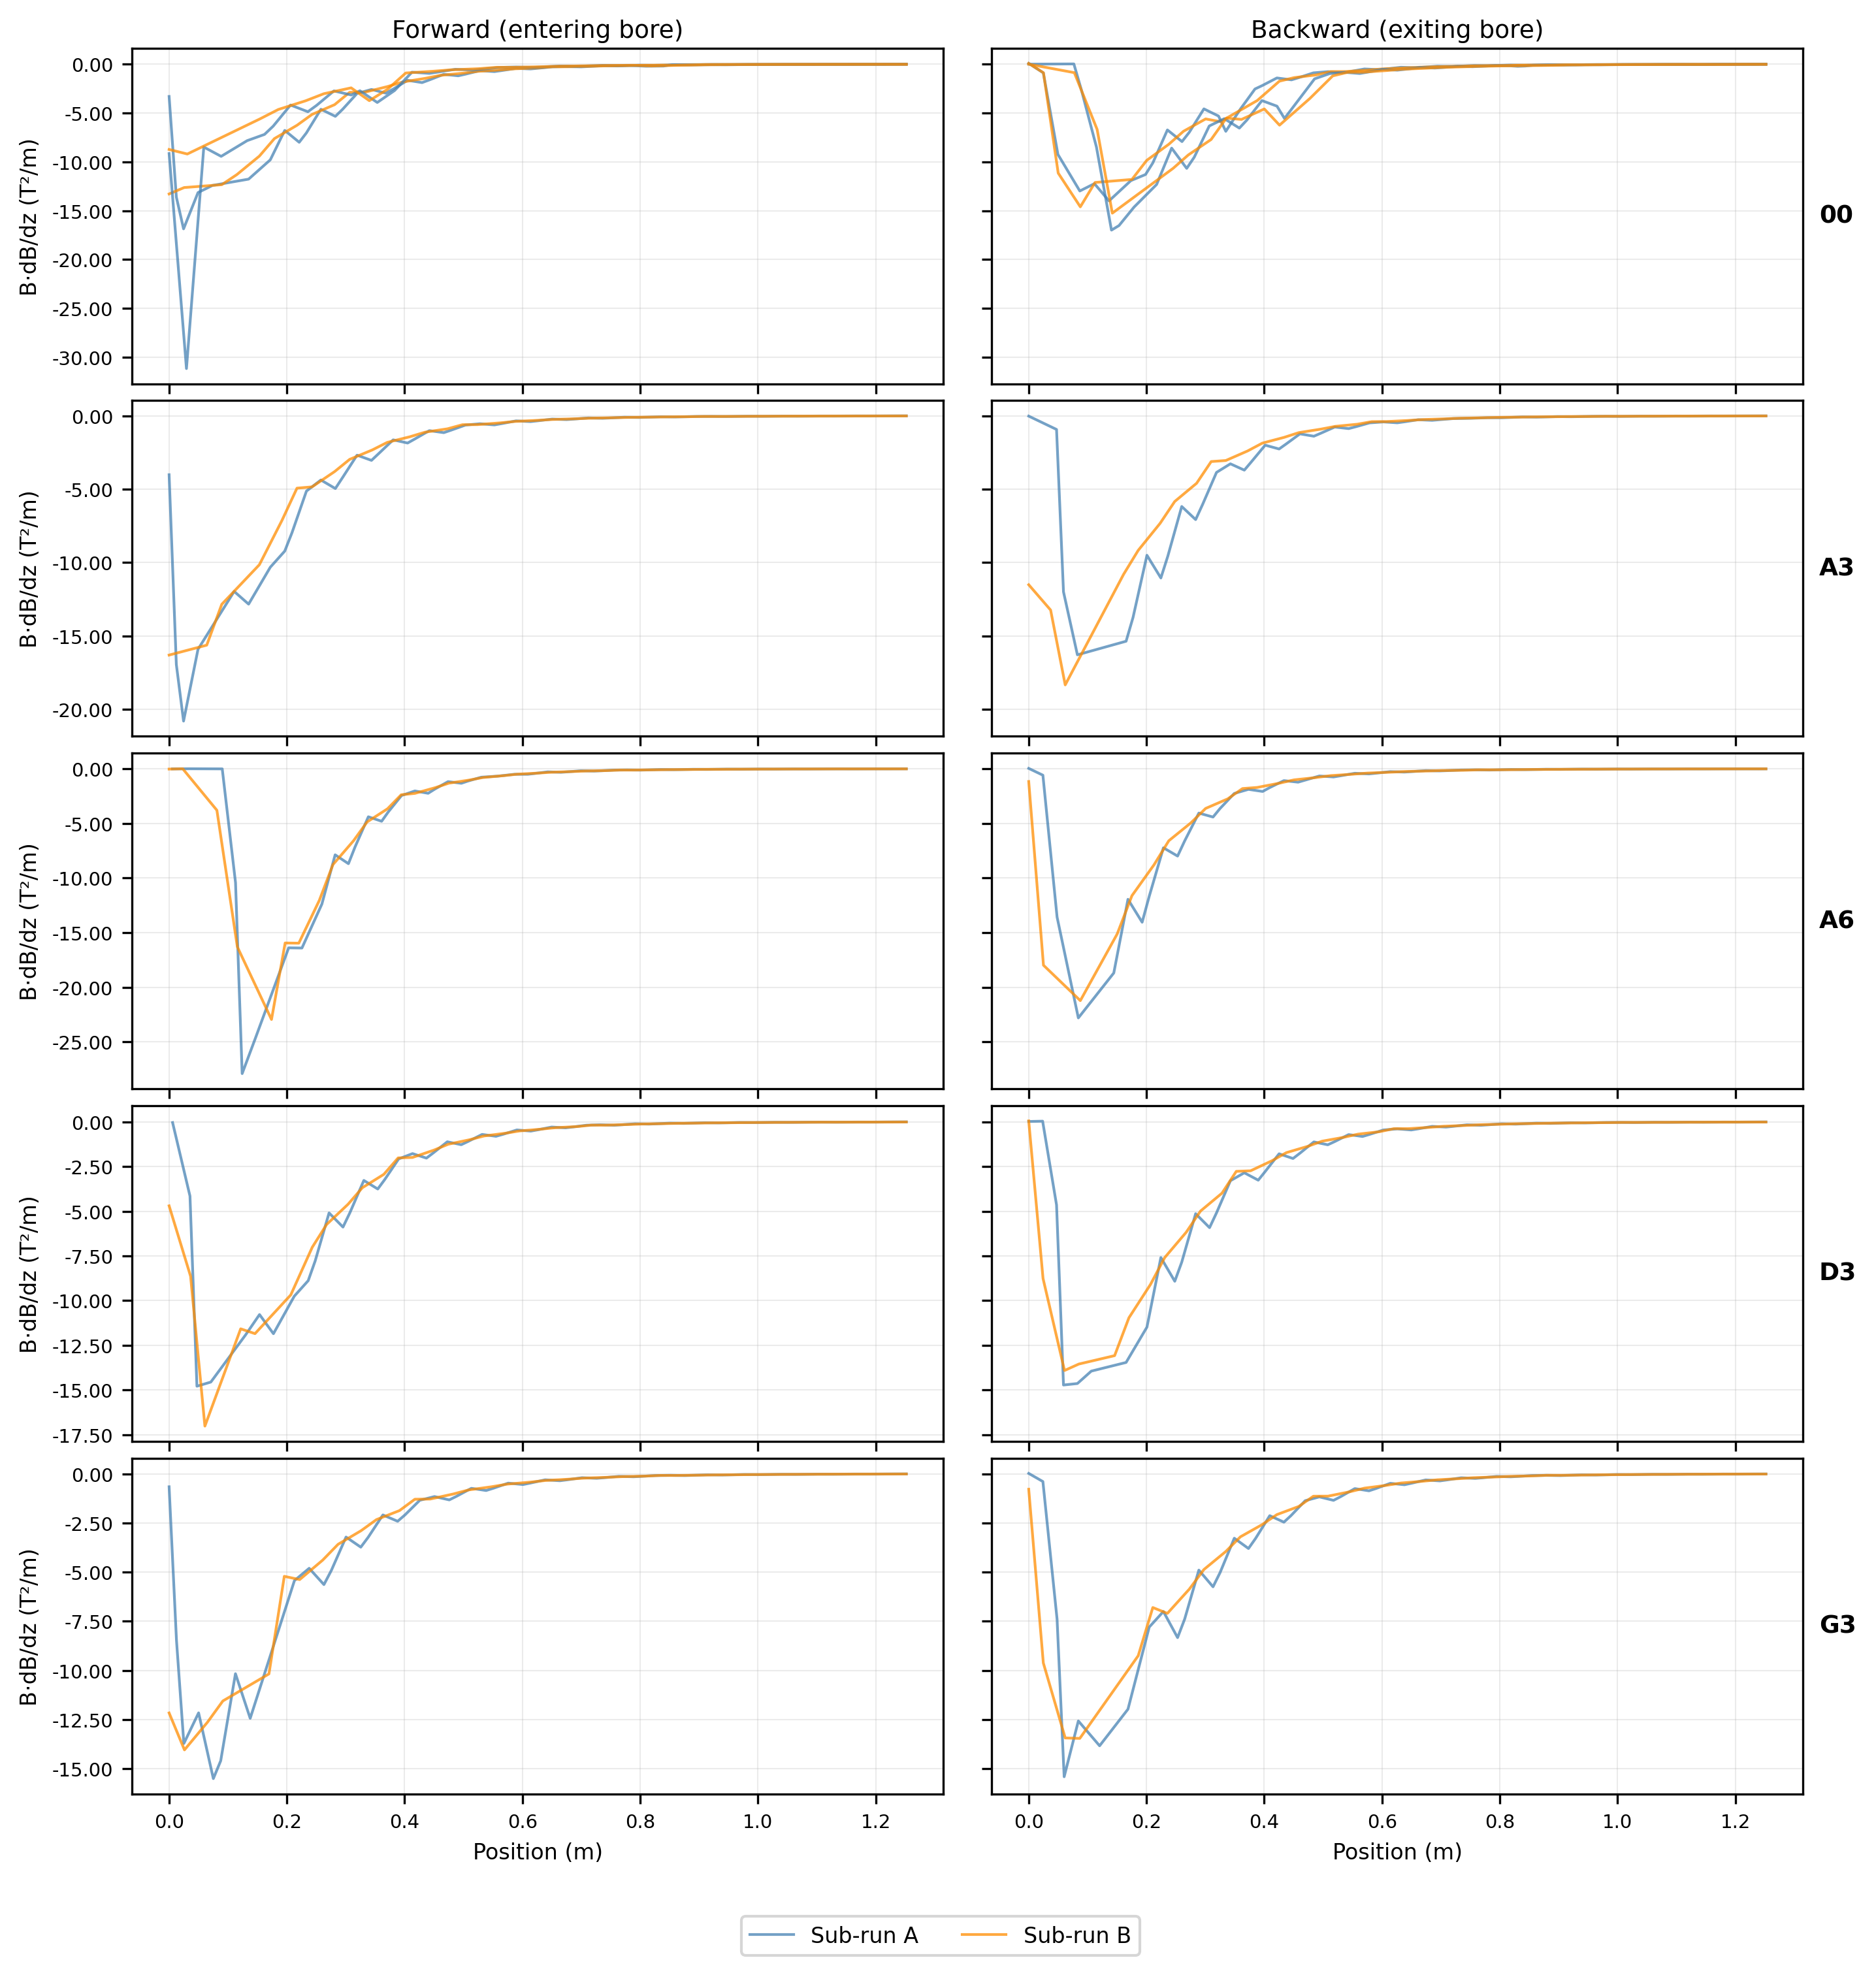
\includegraphics[width=0.85\textwidth]{Assets/allCoords_betterPlots/summary_BgradB.png}
	\caption[Magnetic field and gradient product at all positions separately]{Magnetic field and gradient product along the measurement path}
	\label{fig:allCoords_BgradB}
\end{figure}


\begin{figure}[h!]
	\centering
		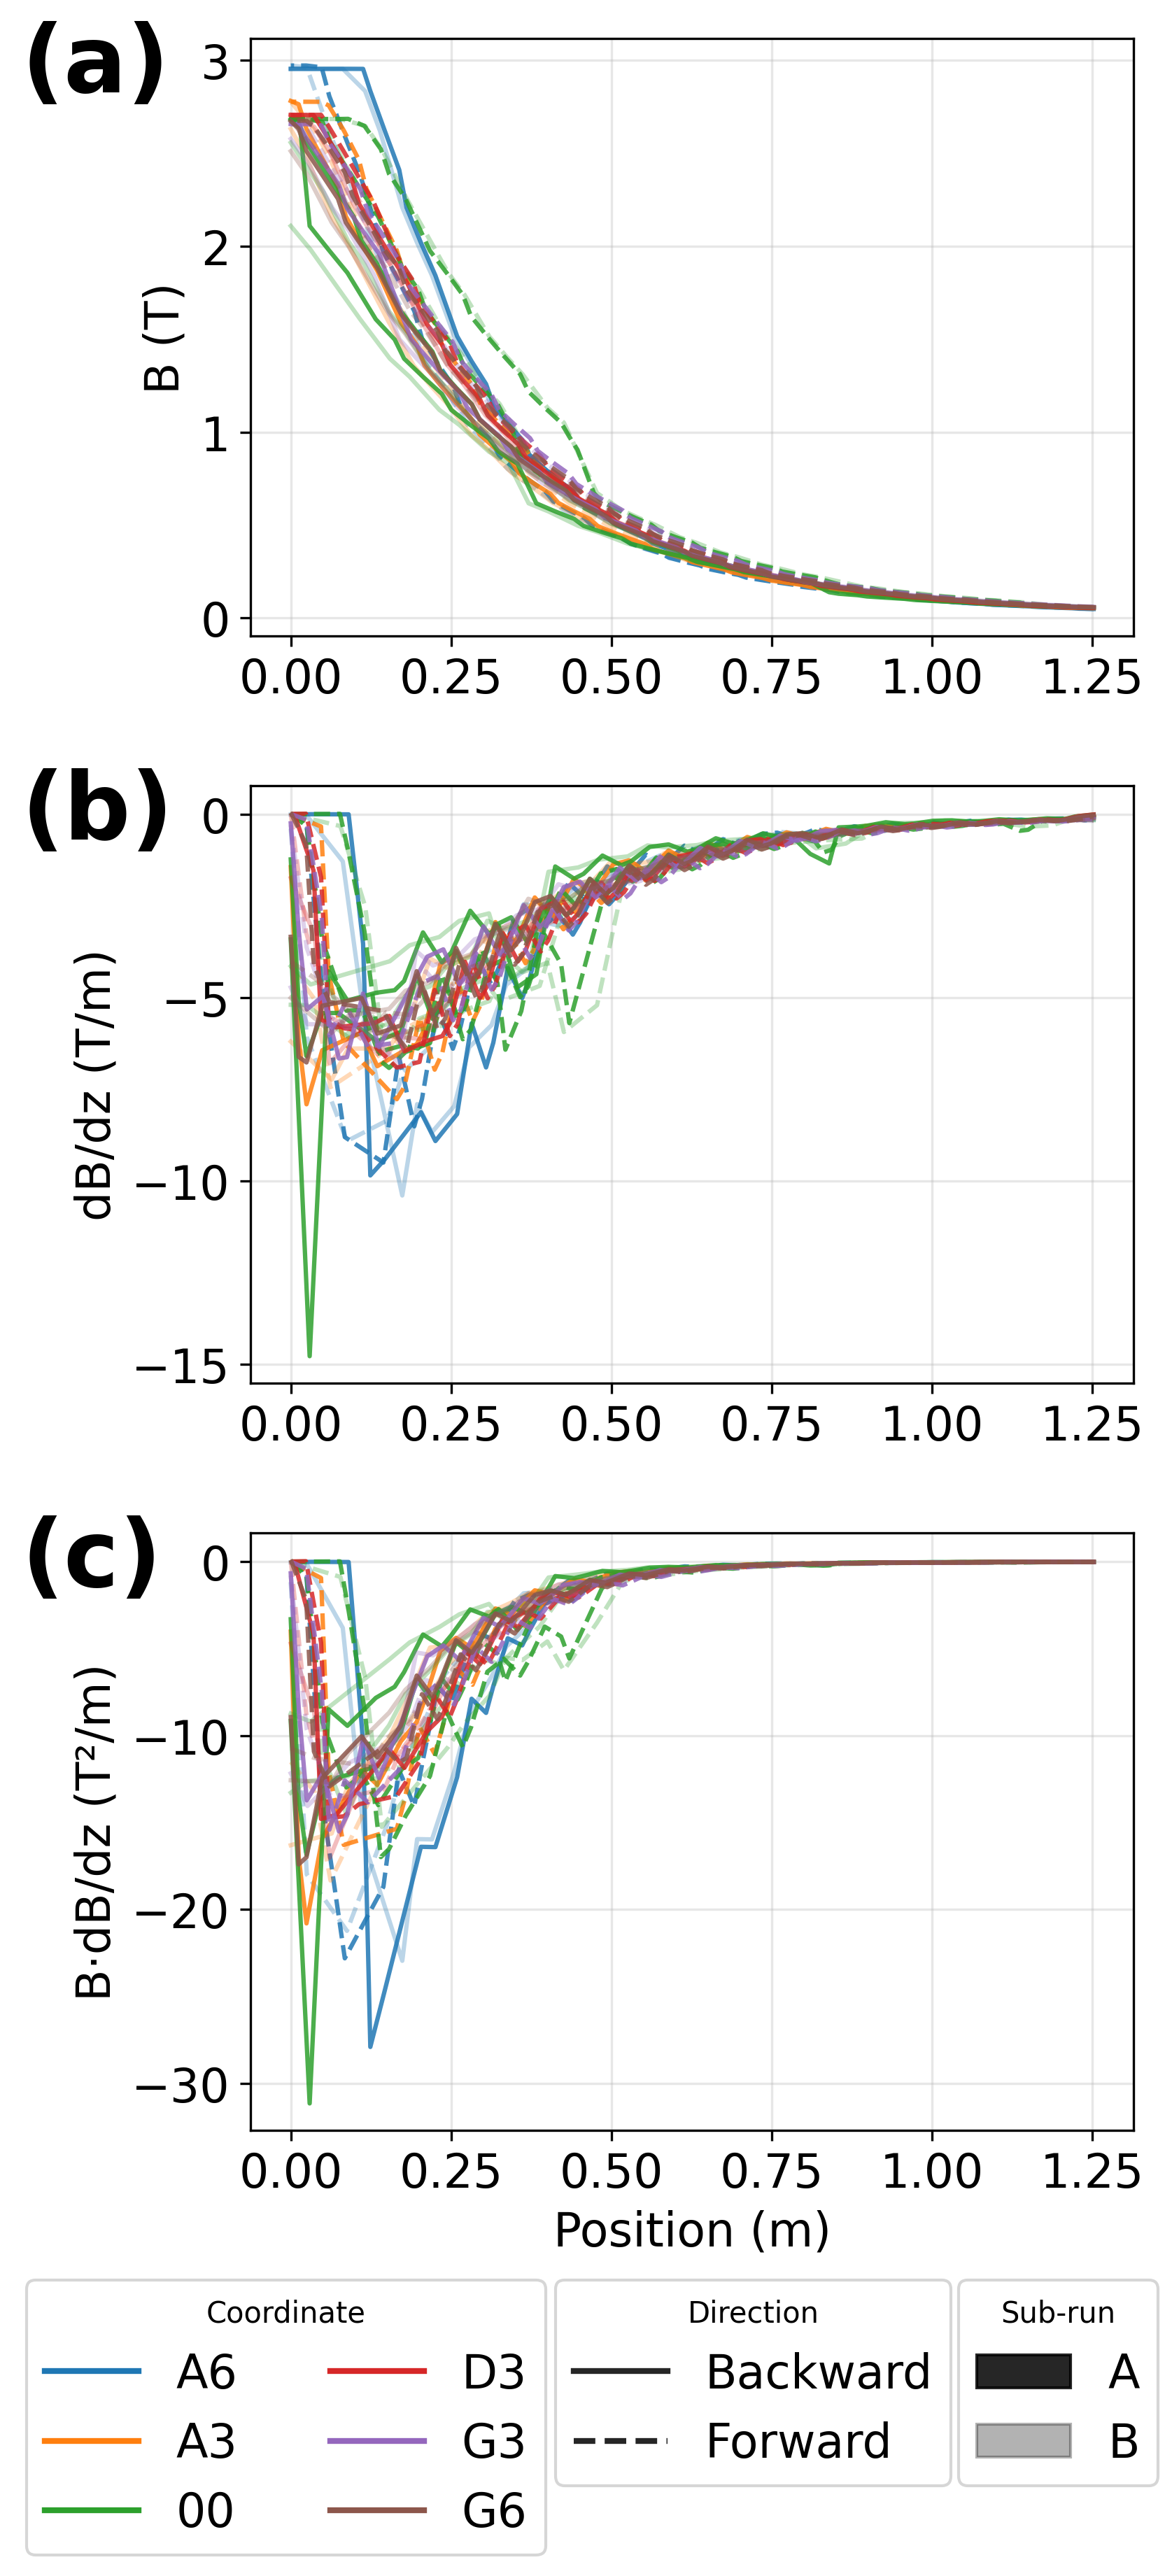
\includegraphics[width=0.65\textwidth]{Assets/allCoords_betterPlots/summary_vertical_overlay_clean.png}
	\caption[Summary of Magnetic field and gradient at all positions]{Magnetic field with corresponding gradient and product along the measurement path. Color represents a coordinate along the fixture A6 is the top, 00 the center and G6 the bottom. Each has two directions, represented with solid/dashed lines, while each direction was split into two sub-runs represented by shade.}
	\label{fig:allCoords_summ}
\end{figure}